% Common preamble for PIGMIE patent figures (A4).
% Drawing conventions:
%   - A4 portrait
%   - Sans-serif throughout (Helvetica)
%   - "Fig. N" sentence-case caption near top
%   - Page "N/total" at top centre
%   - Reference numerals outside boxes via leader lines
%   - ALL CAPS labels in component boxes
%   - Reactor uses north-east-lines hatched fill
%   - Scene uses double-line border
%   - Module enclosures use dashed line with internal numeral

\documentclass[a4paper,10pt]{article}
\usepackage[top=2.5cm,bottom=1.0cm,left=2.5cm,right=1.5cm]{geometry}
\usepackage[T1]{fontenc}
\usepackage{helvet}
\renewcommand{\familydefault}{\sfdefault}
\usepackage{amsmath,amssymb,bm}
\usepackage{tikz}
\usetikzlibrary{shapes,shapes.geometric,shapes.misc,arrows.meta,positioning,fit,calc,backgrounds,decorations.pathreplacing,decorations.markings,patterns}
\pagestyle{empty}
\setlength{\parindent}{0pt}

\tikzset{
  % Component box: ALL CAPS label inside, no numeral inside
  cbox/.style={draw, rectangle, minimum height=1.0cm, minimum width=2.4cm,
               align=center, line width=0.5pt, font=\small},
  cbox-tall/.style={cbox, minimum height=1.6cm},
  cbox-wide/.style={cbox, minimum width=3.0cm},
  cbox-narrow/.style={cbox, minimum width=1.8cm, font=\footnotesize},
  % Reactor / physical medium: hatched fill
  reactor/.style={cbox, pattern=north east lines, pattern color=black!70},
  % Scene: double-line border
  scenebox/.style={cbox, double, double distance=1.2pt, line width=0.4pt},
  % Module / sub-module enclosure
  enclosure/.style={draw, rectangle, dashed, line width=0.4pt, inner sep=10pt, rounded corners=2pt},
  enclosure-solid/.style={draw, rectangle, line width=0.5pt, inner sep=10pt, rounded corners=2pt},
  % Arrows
  flowarr/.style={-Latex, line width=0.5pt, font=\scriptsize},
  flowbi/.style={Latex-Latex, line width=0.5pt, font=\scriptsize},
  flowarr-fb/.style={-Latex, line width=0.5pt, dashed, font=\scriptsize},
  % Reference numeral leader-line endpoint and label
  refnum/.style={font=\footnotesize, inner sep=1pt},
  leader/.style={line width=0.4pt, -Latex},
  % Caption banner
  figcap/.style={font=\bfseries\large}
}

% Helper: figure header (page number + Fig. N caption)
\newcommand{\figheader}[3]{%
  % #1 = page number (e.g. "1"), #2 = total pages, #3 = figure label (e.g. "1" or "4A")
  \noindent\hfill\small #1/#2\hfill\null\par
  \vspace{0.2cm}
  \begin{center}\bfseries Fig.\ #3\end{center}
  \vspace{0.2cm}
}


\begin{document}

\figheader{2}{3}{2}

\begin{center}
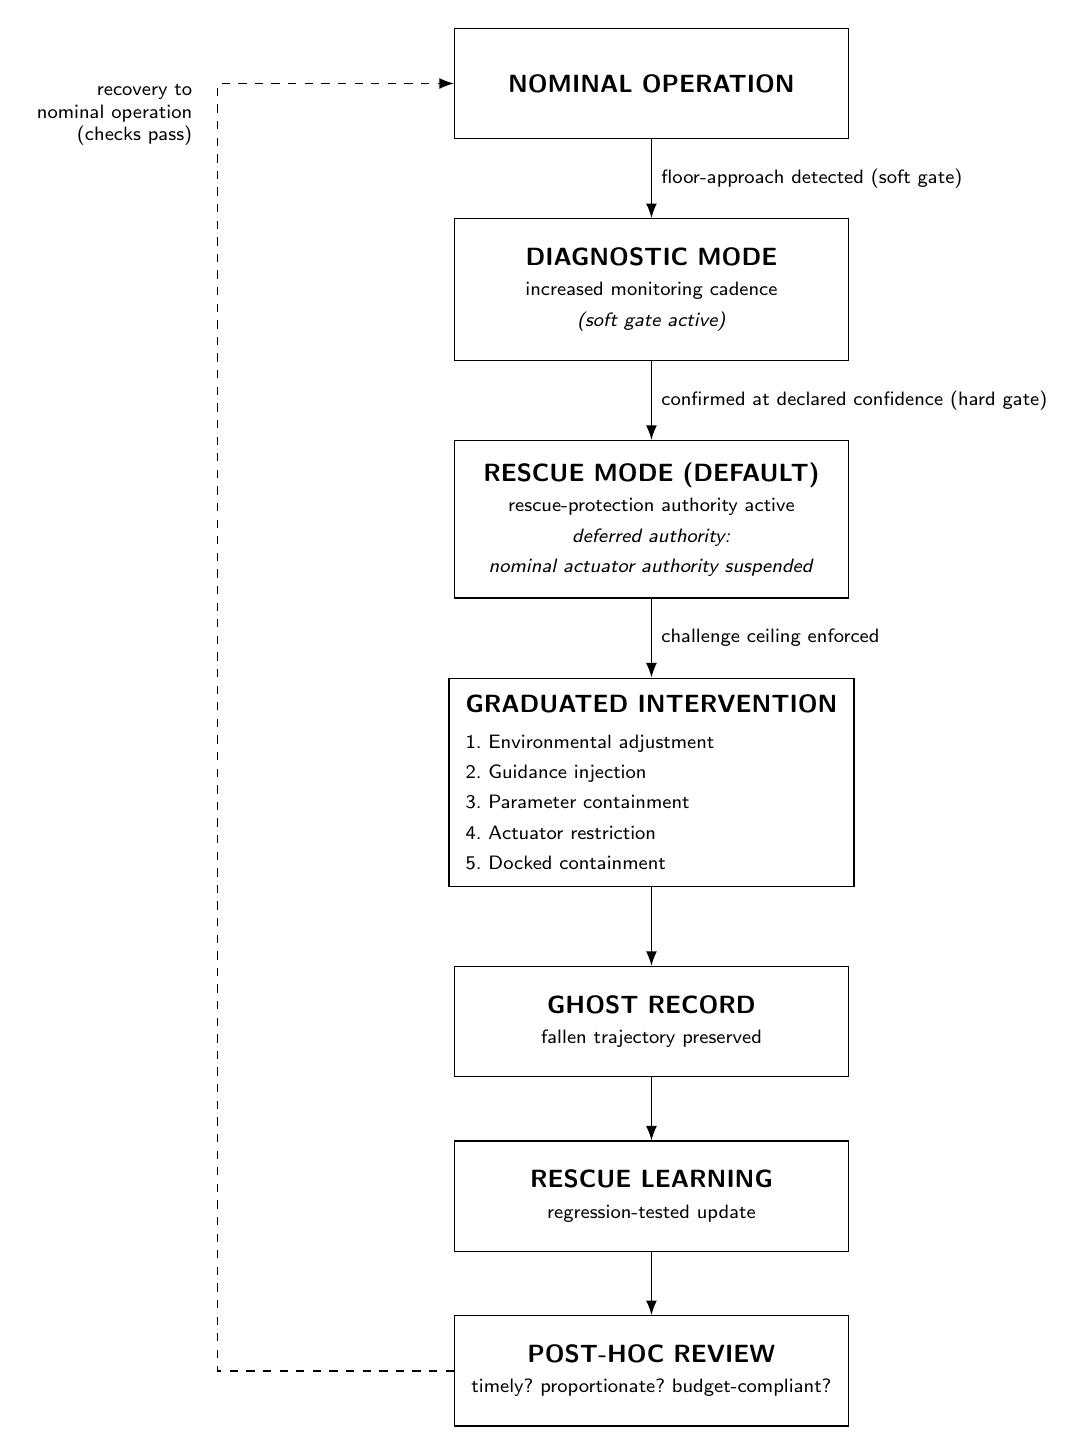
\begin{tikzpicture}[node distance=8mm]

% Vertical flow: Nominal -> Diagnostic (soft-gate) -> Rescue (hard-gate, deferred authority) -> Graduated -> Ghost -> Learn -> Review -> recovery to Nominal

\node[cbox-tall, minimum width=5cm, minimum height=1.4cm] (norm) {\textbf{NOMINAL OPERATION}};
\node[cbox-tall, below=10mm of norm, minimum width=5cm, minimum height=1.8cm] (diag)
  {\textbf{DIAGNOSTIC MODE}\\\scriptsize increased monitoring cadence\\\scriptsize\textit{(soft gate active)}};
\node[cbox-tall, below=10mm of diag, minimum width=5cm, minimum height=2.0cm, align=center] (rescue)
  {\textbf{RESCUE MODE (DEFAULT)}\\\scriptsize rescue-protection authority active\\\scriptsize\textit{deferred authority:}\\\scriptsize\textit{nominal actuator authority suspended}};
\node[cbox-tall, below=10mm of rescue, minimum width=5cm, minimum height=2.6cm, align=left, inner sep=6pt] (grad)
  {\textbf{GRADUATED INTERVENTION}\\[2pt]
   \scriptsize 1.\ Environmental adjustment\\
   \scriptsize 2.\ Guidance injection\\
   \scriptsize 3.\ Parameter containment\\
   \scriptsize 4.\ Actuator restriction\\
   \scriptsize 5.\ Docked containment};
\node[cbox-tall, below=10mm of grad, minimum width=5cm, minimum height=1.4cm] (ghost)
  {\textbf{GHOST RECORD}\\\scriptsize fallen trajectory preserved};
\node[cbox-tall, below=8mm of ghost, minimum width=5cm, minimum height=1.4cm] (learn)
  {\textbf{RESCUE LEARNING}\\\scriptsize regression-tested update};
\node[cbox-tall, below=8mm of learn, minimum width=5cm, minimum height=1.4cm] (review)
  {\textbf{POST-HOC REVIEW}\\\scriptsize timely?\ proportionate?\ budget-compliant?};

% Arrows
\draw[flowarr] (norm.south) -- node[right, font=\scriptsize] {floor-approach detected (soft gate)} (diag.north);
\draw[flowarr] (diag.south) -- node[right, font=\scriptsize] {confirmed at declared confidence (hard gate)} (rescue.north);
\draw[flowarr] (rescue.south) -- node[right, font=\scriptsize] {challenge ceiling enforced} (grad.north);
\draw[flowarr] (grad.south) -- (ghost.north);
\draw[flowarr] (ghost.south) -- (learn.north);
\draw[flowarr] (learn.south) -- (review.north);

% Recovery arrow: post-hoc review back up to nominal operation (closes the loop)
\draw[flowarr-fb] (review.west) -| ++(-30mm,0)
  |- (norm.west);
\node[font=\scriptsize, align=right, anchor=east] at ($(norm.west)+(-32mm,-4mm)$)
  {recovery to\\nominal operation\\(checks pass)};

\end{tikzpicture}
\end{center}

\end{document}
